\documentclass[11pt, letterpaper, journal]{IEEEtran}

\usepackage[utf8]{inputenc}
\usepackage[letterpaper, margin=1.5cm]{geometry}
\usepackage{amsmath}
\usepackage{amssymb}
\usepackage{amsthm}
\usepackage[title]{appendix}
\usepackage{authblk}
\usepackage{cite}
\usepackage[font=scriptsize]{caption}
\usepackage{graphicx}
\usepackage{subcaption}
\usepackage{multicol}
\usepackage{lipsum}
\usepackage{subfig}
\usepackage[dvipsnames]{xcolor}
\usepackage[backend=biber, sorting=ynt]{biblatex}

\addbibresource{bibliography.bib}
\graphicspath{ {./statics/} }
\captionsetup{justification=raggedright, singlelinecheck=false}

\title{Project: Electricity Day-Ahead Price Forecasting}
\author[1]{Ryan Tang}
\affil[1]{Duke University, Statistical Science}
\date{December 5th 2022}

\begin{document}
\maketitle

\section{Introduction}
The electricity market is a peculiar one among all commodities. It is economically non-storable. The power system requires a constant balance between production and consumption. The spot price varies wildly due to temperature, wind speed, sun exposure, and various business and residential activities that exhibit long-term and short-term seasonal patterns. Nevertheless, the world cannot run without electricity. After the deregulation in the 1990s, the introduction of competitive electricity markets reshaped the traditional monopolistic, government-controlled sector. With the wide participation range from public and private generators and distributors to many individual trading firms, the activities have been driving energy prices lower simultaneously, ensuring a stable electricity market. However, forecasting the future electricity price is not a simple endeavor. Utility generators need to do the forecast to plan the production the next day or even the next few years. Distributors need an accurate forecast to satisfy all retail demand in real-time with the lowest price possible. And trading firms need accurate predictions for their arbitrage strategies to drive profitability. Hence, the demand for accurate forecasts is paramount. 

There are two types of forward markets, long-term, and day-ahead. Companies use the long-term markets to plan generation and consumption and hedge risks one to three years ahead. And most of the immediate planning is done in the day-ahead market for the preceding day's retail demand. If there are any differences between the planned load and the realized load, the grid operator often uses the spot market to mark the differences in real-time. The focus of this journal will be the day-ahead market, with its intricacy, where the forecast is delivered one day ahead at once for all 24 hours. In other words, the day-ahead market does not allow continuous trading. Before a specific cutoff time, all bids and offers must be submitted for the next day of each hour. When making the forecast, we have 24 outputs to make.

\begin{figure*}[!h]
\centering
\captionsetup{justification=centering}
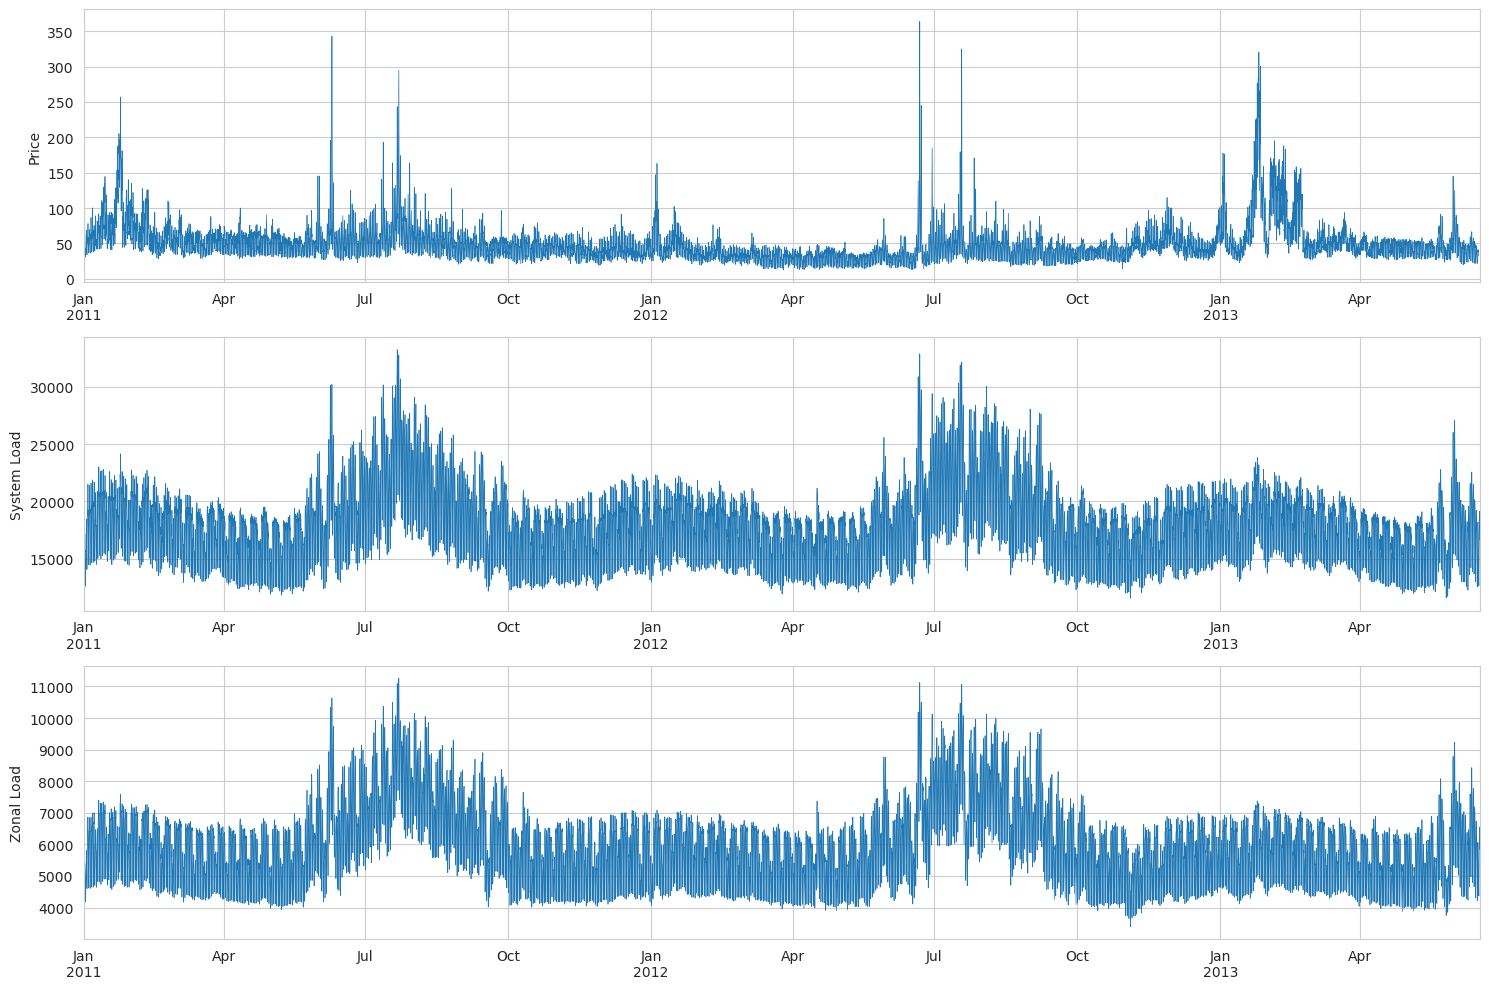
\includegraphics[width=1.0\textwidth]{1.a.png}
\caption{Plots of the electricity price and the two covariates, load estimates.}
\label{fig:competition_data}
\end{figure*}

Hong's team hosted a global energy forecasting competition in 2014 with multiple tracks, GEFCom2014, and open-sourced all the data \cite{HONG2016896}. It has been utilized widely by other researchers as a simple benchmark dataset after that. We, too, will use the same dataset to conduct price forecasting to have a few benchmarks to compare results. The data shown in Figure \ref{fig:competition_data} provided by Hong's team is minimalist, with only 1 price series and 2 co-variate series. In particular, the system load is the forward forecast of consumption or the total amount of energy that needs to be transferred instantaneously on the grid due to demand. Hence, the concept of congestion and grid failure, because when the concurrent amount of electricity on the grid is too high, it overheats the wires and causes congestion and failures. The difference between system and zonal is that zonal only counts the amount of power towards the target zone, and the system counts the total amount of power. Sometimes, a zone can have congestion, and power has to transmit through different wires toward the target zone; therefore, the differences between the two loads also provide signals. Note, here, the price is only the zonal price.

The real-world forecasting task is, in fact, much more complex and takes many other factors into account in the modeling process, such as temperatures, generator failures, transmission congestion, and the inter-dependency of the electricity grid network, which were not present in the dataset. Nevertheless, the data is enough for our purpose.

Not all predictions are treated equally. Due to the inherited volatility of electricity prices, point estimates are often insufficient for energy companies' decision-making and planning process because most transactions are conducted with the forward market. Therefore, coming up with probabilistic predictions is crucial for the task, and it seems to be a natural application for Bayesian analysis. Therefore, here we first formulate the problem as a time series forecasting under certainty by utilizing probabilistic modeling, applying Hidden Markov Model (HMM) to the problem, and comparing it with a few empirical results presented in Nowotarski's paper \cite{NOWOTARSKI20181548}. In the last section, we perform diagnostics on HMM and propose future improvements.


\section{Previous Work}
Despite its importance, electric price forecasting (EPF) is an underdeveloped and often overlooked research area \cite{NOWOTARSKI20181548}. The publication pace had only started to pick up attention since 2000, the California crisis. And the pace had only started to pick up since 2005. Many publications focus on using neural networks in prediction, some utilize classic time series methodologies, but the majority concentrates on point forecasting. As we highlighted the importance of probabilistic electric price forecasting forecast (PEPF) previously, it is, even more, an undeveloped regime and barely picks up the pace since 2011.

Weron has extensively reviewed various models used in EPF literature and their relative strengths and weaknesses \cite{WERON20141030}. He segmented all modeling approaches into 5 categories, but we think 3 are more appropriate because of their significant overlap. The multi-agent model is the first segment that has its root in game theory. It tries to model market competition, supply and demand, and many other fundamental factors by formulating equilibrium and a strategic game. Such formulation is neat for theoretical pursuit and creating beautiful theorem but lacks a general solution except for some toy examples. And often, such a method relies on fundamental data and only updates weekly, monthly, or even yearly, making them unsuitable for day-ahead prediction. The second major segment consists of many traditional models, including many variants of neural networks, support vector machines, random forests, gradient boosting machines, etc. These model are great point predictor that works well with non-linearity. However, there has not been a thorough investigation of these methods, according to Weron, because it is difficult to establish a benchmark due to the temporal nature of the task. The last segment consists of many statistical and probabilistic models, including the classic time series models, AR, ARX, GARCH, regression, and Markovian models like Jump Diffusion and Markov-Regime Switching. Weron summarized the former tends to perform poorly on sudden spikes, and the latter tends to capture spikes and volatility quite well but lacks forward predictability. We believe the statement is biased because they never considered Bayesian analysis in the context.

We introduce two classic benchmarks for comparison purposes, which we will briefly discuss in this section. Although most methods discussed by Weron to date only offer point estimations by design, many auxiliary techniques can be utilized to construct a prediction interval. We also introduce one of the most straightforward methods, historical simulation, too, in this section. So we can make a comparison between the benchmarks and our method coherently.

\subsection{Benchmark}
We called this the naive model because it simply uses the last day or week's hourly price for the current estimates based on the day of the week. Namely, $$\hat{P}_{d,h} = P_{d-1, h}$$ on Tuesday, Wednesday, Thursday or Friday, and $$\hat{P}_{d,h} = P_{d-7, h}$$ on Monday, Saturday, or Sunday. We used the conventional electricity price notation here that $P_{d,h}$ stands for the electricity price at day $d$ hour $h$; hence $P_{d-1, h}$ is the $h$-th hourly price from yesterday. Obviously, there is no training or parameter to tune except that we need a week's data for initial calibration.

\subsection{Autoregressive Model (ARX)}
Another popular model that are adopted widely in the community uses an autoregressive (AR) model with extra factors (ARX), X stands for exogenous variables. Simply put, it is a linear regression on AR. Misiorek et al. introduced it originally, and the model uses a centered log-price $p_{d,h}$, few autoregressive lag terms, log zonal load $z_{d,h}$, and day of week effects $D_{day}$ which follow the following equation:
\begin{align*}
    p_{d,h} &= \log(P_{d,h}) - \frac{1}{T}\sum_{t=1}^{T} \log(P_{t, h}) \\
    \hat{p}_{d,h} &= \beta_h^{\intercal} x_{d,h} \\
    x_{d, h} &= (p_{d-1,h}, p_{d-2,h}, p_{d-7,h}, p_{d-1}^{min}, \\
             &\quad \,\,\, z_{d,h}, D_{sat}, D_{sun}, D_{mon})^{\intercal}
\end{align*}
Here $T$ is the model calibration, or training, period which was chosen as 365 days. The day of week effects were handled using one-hot-encoding in our case for only Monday, Sunday, and Saturday.

\subsection{Prediction Interval {PI} Construction}
The interval bounds are usually determined simply using historical residual analysis. Hence, the prediction interval, $[\hat{L}_t, \hat{U}_t]$, lower and upper bounds are estimated directly using the observed prediction errors $\epsilon_t$ with the respective quantile in the training sets. 
\begin{align*}
    \epsilon_t &= P_t - \hat{P}_t \\
    \hat{L}_t &= \hat{P}_t + \hat{F}^{-1}_{\epsilon, t}(1-q) \\
    \hat{U}_t &= \hat{P}_t + \hat{F}^{-1}_{\epsilon, t}(q)
\end{align*}
where $\hat{F}^{-1}_{\epsilon, t}(\cdot)$ is the inverse CDF function of the empirical prediction residual at time $t$ and $q$ is the quantile in interest, and $\hat{P}_t$ is the predicted electricity price at time $t$. We used this methodology to construct the PI for all the benchmark models.


\section{Evaluation Metrics}
We are spitting out full probability distribution rather than a point estimate. However, the realization is a scalar. We need a specific way of assessing the performance of the probabilistic prediction in this context. The goal is to maximize sharpness while maintaining calibration. Calibration is crucial because we like to ensure the outputted distribution reflects the true, observed density. It is often time called unbiasedness. On the other hand, sharpness concerns the prediction variances, often called precision; the tighter the distribution, the better. Below, we introduce two widely used metrics for performance evaluations that will be used in our performance evaluations.

\subsection{Unconditional coverage (UC)}
The intuition behind this metric is that the ideal empirical coverage of the quantile should resemble to the nominal quantile coverage. Here, we first introduce the hits and misses indicator $\mathbf{1}_t$ for every prediction at time $t$. Then, the unconditional coverage of our series of probabilistic prediction, UC, is defined as below.
\begin{align*}
    \mathbf{1}_t &= \begin{cases}
        1 & \text{if $\hat{P}_t \in [\hat{L}_t, \hat{U}_t]$} \\
        0 & \text{otherwise} \\
    \end{cases} \\
    UC &= \frac{1}{T}\sum_{t=1}^T \mathbf{1}_t
\end{align*}

\subsection{Continuous Ranked Probability Score (CRPS)}
In a nutshell, CRPS measures how closer a predicted distribution to a delta function that centers at the observed instance; the smaller the value the better and is defined as $$CRPS(\hat{F}_{P_t}, P_t) = \int_{-\infty}^{\infty} (\hat{F}_{P_t} - \mathbf{1}_{\{P_t \leq x\}})^2 dx$$ However, the integral is hard to estimate. Often, we have to rely on approximation. One useful way is to use a series Pinball loss at different quantile ranging from 1\% to 99\% then average them up to arrive on the approximation. Pinball loss is an asymmetric linear loss version of L1-loss. Instead of calculating the loss at the median, 50-th quantile, it does on any arbitrary point. Hence, it is often called the quantile loss.
\begin{align*}
    Pinball&(\hat{Q}_{P_t}(q), P_t, q) \\&= \begin{cases}
        (1-q) |\hat{Q}_{P_t}(q) - P_t| & \text{if $P_t < \hat{Q}_{P_t}(q)$} \\
        q |\hat{Q}_{P_t}(q) - P_t| & \text{if $P_t \geq \hat{Q}_{P_t}(q)$} \\
    \end{cases} \\
    CRPS&(\hat{F}_{P_t}, P_t) = \int_{0}^{1} Pinball(\hat{Q}_{P_t}(q), P_t, q) dq
\end{align*}
$\hat{Q}_{P_t}(q)$ is the price forecast at the q-th quantile and $P_t$ is the observed price. We can see when $q=0.5$, the Pinball loss reduces to the L1-loss.


\section{Problem Formulation}
In this section, we define the exact formulation of the proposed HMM model. Rather than relying on the historical simulation method for constructing the prediction interval, we uses a forward sampling directly through the posterior predictive distribution using Markov Chain Monte Carlo (MCMC) which comes naturally through our graphical model and is one of the biggest advantage on using Bayesian method to quantify uncertainty directly in terms of posterior. Like all HMM, the model consists of a discrete hidden state denoted $Z_t \in \{0, 1\}$, a conditional observation model, $p(y_t|Z=z_k, x_t)$, and a transition matrix $A$. Here we assumes time invariant $A$, but parameterized the observation model using Gaussian distribution with $\theta_k=(\beta_k, \sigma_k^2)$ conditionally independent of each hidden state $k$. Lastly, we placed priors on top all of them for Bayesian methods. Mathematically, the following is the model specs.
\begin{align*}
    p(z_0) &= p(\pi) \\
    p(z_t|z_{t-1}) &= A_{ji} \\
    p(y_t|x_i, Z_t=z_k) &= \mathcal{N}(y_t|x_i^{\intercal}\beta_k, \sigma^2_k) \\
    A_{j\cdot} &\thicksim Dir({\alpha_1, ..., \alpha_k}) \\
    \beta_k &\thicksim \mathcal{N}(\mu_{ko}=0, \sigma^2_{ko}=100) \\
    1/\sigma^2_{k} &\thicksim Gamma(1, 20)
\end{align*}
Note, we decided to only assume two hidden states. One because it already captures the spiky phenomenal quite well, we have limited amount of data, and too many hidden states quickly exacerbate the sampling speed. Hence, the transition matrix is $A \in \mathbf{R}^{2\times 2}$ and we model the each row with its Dirichlet prior. For the design matrix, we decided to use the same features from the ARX model which contains 8 expert selected features, $\beta_k \in \mathbf{R}^8$. And, follows the typical full-conditional of a Bayesian linear regression model, we pick the normal prior for $\beta_k$ and gamma prior for the precision $1/\sigma^2_k$. Lastly, we fit the model individually for each hourly time series, but we can still compactly write it still using a multivariate-normal with a diagonalized covariance matrix $\sigma^2\mathbf{I}_k$. Therefore, the resulting model consists one for each hour, in total contains 528 parameters, 22 per hour.


$p(y|Z=z_k, x) \thicksim N(\mu$  The Baum-Welch algorithm, specially, the forward filtering backward sampling algorithm is used in MCMC sampling because we don't 


\section{Results \& Diagnostics}
Compare the GM-HMM result to the benchmark, AR, and QRA in terms of UC and CRPS.

\section{Conclusions}

\printbibliography[heading=bibintoc, title={References}]


\end{document}